%% abtex2-modelo-trabalho-academico.tex, v-1.9.2 laurocesar
%% Copyright 2012-2014 by abnTeX2 group at http://abntex2.googlecode.com/ 
%%
%% This work may be distributed and/or modified under the
%% conditions of the LaTeX Project Public License, either version 1.3
%% of this license or (at your option) any later version.
%% The latest version of this license is in
%%   http://www.latex-project.org/lppl.txt
%% and version 1.3 or later is part of all distributions of LaTeX
%% version 2005/12/01 or later.
%%
%% This work has the LPPL maintenance status `maintained'.
%% 
%% The Current Maintainer of this work is the abnTeX2 team, led
%% by Lauro César Araujo. Further information are available on 
%% http://abntex2.googlecode.com/
%%
%% This work consists of the files abntex2-modelo-trabalho-academico.tex,
%% abntex2-modelo-include-comandos and abntex2-modelo-references.bib
%%

% ------------------------------------------------------------------------
% ------------------------------------------------------------------------
% abnTeX2: Modelo de Trabalho Academico (tese de doutorado, dissertacao de
% mestrado e trabalhos monograficos em geral) em conformidade com 
% ABNT NBR 14724:2011: Informacao e documentacao - Trabalhos academicos -
% Apresentacao
% ------------------------------------------------------------------------
% ------------------------------------------------------------------------

\documentclass[
	% -- opções da classe memoir --
	12pt,				% tamanho da fonte
	openright,			% capítulos começam em pág ímpar (insere página vazia caso preciso)
	twoside,			% para impressão em verso e anverso. Oposto a oneside
	a4paper,			% tamanho do papel. 
	% -- opções da classe abntex2 --
	%chapter=TITLE,		% títulos de capítulos convertidos em letras maiúsculas
	%section=TITLE,		% títulos de seções convertidos em letras maiúsculas
	%subsection=TITLE,	% títulos de subseções convertidos em letras maiúsculas
	%subsubsection=TITLE,% títulos de subsubseções convertidos em letras maiúsculas
	% -- opções do pacote babel --
	english,			% idioma adicional para hifenização
	brazil				% o último idioma é o principal do documento
	]{abntex2}

% ---
% Pacotes básicos 
% ---
\usepackage{lmodern}			% Usa a fonte Latin Modern			
\usepackage[T1]{fontenc}		% Selecao de codigos de fonte.
\usepackage[utf8]{inputenc}		% Codificacao do documento (conversão automática dos acentos)
\usepackage{lastpage}			% Usado pela Ficha catalográfica
\usepackage{indentfirst}		% Indenta o primeiro parágrafo de cada seção.
\usepackage{color}				% Controle das cores
\usepackage{graphicx}			% Inclusão de gráficos
\usepackage{microtype} 			% para melhorias de justificação
% ---
		

% ---
% Pacotes de citações
% ---
\usepackage[brazilian,hyperpageref]{backref}	 % Paginas com as citações na bibl
\usepackage[num]{abntex2cite}	% Citações padrão ABNT
\citebrackets[]
% --- 
% CONFIGURAÇÕES DE PACOTES
% --- 

% ---
% Configurações do pacote backref
% Usado sem a opção hyperpageref de backref
\renewcommand{\backrefpagesname}{Citado na(s) página(s):~}
% Texto padrão antes do número das páginas
\renewcommand{\backref}{}
% Define os textos da citação
\renewcommand*{\backrefalt}[4]{
	\ifcase #1 %
		Nenhuma citação no texto.%
	\or
		Citado na página #2.%
	\else
		Citado #1 vezes nas páginas #2.%
	\fi}%
% ---

% ---
% Informações de dados para CAPA e FOLHA DE ROSTO
% ---
\titulo{Chuveiro com aquecimento indutivo}
\autor{Igor Macedo Quintanilha\\ Roberto de Moura Estevão Filho}
\local{Rio de Janeiro}
\data{2013}
\orientador{Carlos José Ribas D'Avila}
\coorientador{Joarez Bastos Monteiro}
\instituicao{%
  Universidade Federal do Rio de Janeiro
  \par
  Escola Politécnica
  \par
  Departamento de Engenharia Eletrônica
  \par
  Projeto Integrado}
\tipotrabalho{Trabalho}
% O preambulo deve conter o tipo do trabalho, o objetivo, 
% o nome da instituição e a área de concentração 
\preambulo{Trabalho realizado para a disciplina Projeto Integrado do curso de Engenharia Eletrônica da Universidade Federal do Rio de Janeiro}
% ---


% ---
% Configurações de aparência do PDF final

% alterando o aspecto da cor azul
\definecolor{blue}{RGB}{41,5,195}

% informações do PDF
\makeatletter
\hypersetup{
     	%pagebackref=true,
		pdftitle={\@title}, 
		pdfauthor={\@author},
    	pdfsubject={\imprimirpreambulo},
	    pdfcreator={LaTeX with abnTeX2},
		pdfkeywords={abnt}{latex}{abntex}{abntex2}{trabalho acadêmico}, 
		colorlinks=true,       		% false: boxed links; true: colored links
    	linkcolor=blue,          	% color of internal links
    	citecolor=blue,        		% color of links to bibliography
    	filecolor=magenta,      		% color of file links
		urlcolor=blue,
		bookmarksdepth=4
}
\makeatother
% --- 

% --- 
% Espaçamentos entre linhas e parágrafos 
% --- 

% O tamanho do parágrafo é dado por:
\setlength{\parindent}{1.3cm}

% Controle do espaçamento entre um parágrafo e outro:
\setlength{\parskip}{0.2cm}  % tente também \onelineskip

% ---
% compila o indice
% ---
\makeindex
% ---

% ----
% Início do documento
% ----
\begin{document}


% Retira espaço extra obsoleto entre as frases.
\frenchspacing 

% ----------------------------------------------------------
% ELEMENTOS PRÉ-TEXTUAIS
% ----------------------------------------------------------
% \pretextual

% ---
% Capa
% ---
\imprimircapa
% ---

% ---
% Folha de rosto
% (o * indica que haverá a ficha bibliográfica)
% ---
\imprimirfolhaderosto*
% ---

% ---
% Inserir a ficha bibliografica
% ---

% Isto é um exemplo de Ficha Catalográfica, ou ``Dados internacionais de
% catalogação-na-publicação''. Você pode utilizar este modelo como referência. 
% Porém, provavelmente a biblioteca da sua universidade lhe fornecerá um PDF
% com a ficha catalográfica definitiva após a defesa do trabalho. Quando estiver
% com o documento, salve-o como PDF no diretório do seu projeto e substitua todo
% o conteúdo de implementação deste arquivo pelo comando abaixo:
%
% \begin{fichacatalografica}
%     \includepdf{fig_ficha_catalografica.pdf}
% \end{fichacatalografica}
%\begin{fichacatalografica}
%	\vspace*{\fill}					% Posição vertical
%	\hrule							% Linha horizontal
%	\begin{center}					% Minipage Centralizado
%	\begin{minipage}[c]{12.5cm}		% Largura
%	
%	\imprimirautor
%	
%	\hspace{0.5cm} \imprimirtitulo  / \imprimirautor. --
%	\imprimirlocal, \imprimirdata-
%	
%	\hspace{0.5cm} \pageref{LastPage} p. : il. (algumas color.) ; 30 cm.\\
%	
%	\hspace{0.5cm} \imprimirorientadorRotulo~\imprimirorientador\\
%	
%	\hspace{0.5cm}
%	\parbox[t]{\textwidth}{\imprimirtipotrabalho~--~\imprimirinstituicao,
%	\imprimirdata.}\\
%	
%	\hspace{0.5cm}
%		1. Palavra-chave1.
%		2. Palavra-chave2.
%		I. Orientador.
%		II. Universidade xxx.
%		III. Faculdade de xxx.
%		IV. Título\\ 			
%	
%	\hspace{8.75cm} CDU 02:141:005.7\\
%	
%	\end{minipage}
%	\end{center}
%	\hrule
%\end{fichacatalografica}
% ---

% ---
% Inserir errata
% ---
%\begin{errata}
%Elemento opcional da \citeonline[4.2.1.2]{NBR14724:2011}. Exemplo:
%
%\vspace{\onelineskip}
%
%FERRIGNO, C. R. A. \textbf{Tratamento de neoplasias ósseas apendiculares com
%reimplantação de enxerto ósseo autólogo autoclavado associado ao plasma
%rico em plaquetas}: estudo crítico na cirurgia de preservação de membro em
%cães. 2011. 128 f. Tese (Livre-Docência) - Faculdade de Medicina Veterinária e
%Zootecnia, Universidade de São Paulo, São Paulo, 2011.
%
%\begin{table}[htb]
%\center
%\footnotesize
%\begin{tabular}{|p{1.4cm}|p{1cm}|p{3cm}|p{3cm}|}
%  \hline
%   \textbf{Folha} & \textbf{Linha}  & \textbf{Onde se lê}  & \textbf{Leia-se}  \\
%    \hline
%    1 & 10 & auto-conclavo & autoconclavo\\
%   \hline
%\end{tabular}
%\end{table}
%
%\end{errata}
% ---

% ---
% Inserir folha de aprovação
% ---

% Isto é um exemplo de Folha de aprovação, elemento obrigatório da NBR
% 14724/2011 (seção 4.2.1.3). Você pode utilizar este modelo até a aprovação
% do trabalho. Após isso, substitua todo o conteúdo deste arquivo por uma
% imagem da página assinada pela banca com o comando abaixo:
%
% \includepdf{folhadeaprovacao_final.pdf}
%
\begin{folhadeaprovacao}

  \begin{center}
    {\ABNTEXchapterfont\large\imprimirautor}

    \vspace*{\fill}\vspace*{\fill}
    \begin{center}
      \ABNTEXchapterfont\bfseries\Large\imprimirtitulo
    \end{center}
    \vspace*{\fill}
    
    \hspace{.45\textwidth}
    \begin{minipage}{.5\textwidth}
        \imprimirpreambulo
    \end{minipage}%
    \vspace*{\fill}
   \end{center}
        

   \assinatura{\textbf{\imprimirorientador} \\ Orientador} 
   \assinatura{Joarez Bastos Monteiro \\ Coorientador}
      
   \begin{center}
    \vspace*{0.5cm}
    {\large\imprimirlocal}
    \par
    {\large\imprimirdata}
    \vspace*{1cm}
  \end{center}
  
\end{folhadeaprovacao}
% ---

% ---
% Dedicatória
% ---
%\begin{dedicatoria}
%   \vspace*{\fill}
%   \centering
%   \noindent
%   \textit{ Este trabalho é dedicado às crianças adultas que,\\
%   quando pequenas, sonharam em se tornar cientistas.} \vspace*{\fill}
%\end{dedicatoria}
% ---

% ---
% Agradecimentos
% ---
%\begin{agradecimentos}
%Os agradecimentos principais são direcionados à Gerald Weber, Miguel Frasson,
%Leslie H. Watter, Bruno Parente Lima, Flávio de Vasconcellos Corrêa, Otavio Real
%Salvador, Renato Machnievscz\footnote{Os nomes dos integrantes do primeiro
%projeto abn\TeX\ foram extraídos de
%\url{http://codigolivre.org.br/projects/abntex/}} e todos aqueles que
%contribuíram para que a produção de trabalhos acadêmicos conforme
%as normas ABNT com \LaTeX\ fosse possível.
%
%Agradecimentos especiais são direcionados ao Centro de Pesquisa em Arquitetura
%da Informação\footnote{\url{http://www.cpai.unb.br/}} da Universidade de
%Brasília (CPAI), ao grupo de usuários
%\emph{latex-br}\footnote{\url{http://groups.google.com/group/latex-br}} e aos
%novos voluntários do grupo
%\emph{\abnTeX}\footnote{\url{http://groups.google.com/group/abntex2} e
%\url{http://abntex2.googlecode.com/}}~que contribuíram e que ainda
%contribuirão para a evolução do \abnTeX.
%
%\end{agradecimentos}
% ---

% ---
% Epígrafe
% ---
%\begin{epigrafe}
%    \vspace*{\fill}
%	\begin{flushright}
%		\textit{``Não vos amoldeis às estruturas deste mundo, \\
%		mas transformai-vos pela renovação da mente, \\
%		a fim de distinguir qual é a vontade de Deus: \\
%		o que é bom, o que Lhe é agradável, o que é perfeito.\\
%		(Bíblia Sagrada, Romanos 12, 2)}
%	\end{flushright}
%\end{epigrafe}
% ---

% ---
% RESUMOS
% ---

% resumo em português
%\setlength{\absparsep}{18pt} % ajusta o espaçamento dos parágrafos do resumo
%\begin{resumo}
% Segundo a \citeonline[3.1-3.2]{NBR6028:2003}, o resumo deve ressaltar o
% objetivo, o método, os resultados e as conclusões do documento. A ordem e a extensão
% destes itens dependem do tipo de resumo (informativo ou indicativo) e do
% tratamento que cada item recebe no documento original. O resumo deve ser
% precedido da referência do documento, com exceção do resumo inserido no
% próprio documento. (\ldots) As palavras-chave devem figurar logo abaixo do
% resumo, antecedidas da expressão Palavras-chave:, separadas entre si por
% ponto e finalizadas também por ponto.
%
% \textbf{Palavras-chaves}: latex. abntex. editoração de texto.
%\end{resumo}
%
%% resumo em inglês
%\begin{resumo}[Abstract]
% \begin{otherlanguage*}{english}
%   This is the english abstract.
%
%   \vspace{\onelineskip}
% 
%   \noindent 
%   \textbf{Key-words}: latex. abntex. text editoration.
% \end{otherlanguage*}
%\end{resumo}


% ---
% inserir lista de ilustrações
% ---
\pdfbookmark[0]{\listfigurename}{lof}
\listoffigures*
\cleardoublepage
% ---

% ---
% inserir lista de tabelas
% ---
\pdfbookmark[0]{\listtablename}{lot}
\listoftables*
\cleardoublepage
% ---

% ---
% inserir lista de abreviaturas e siglas
% ---
%\begin{siglas}
%  \item[ABNT] Associação Brasileira de Normas Técnicas
%  \item[abnTeX] ABsurdas Normas para TeX
%\end{siglas}
% ---

% ---
% inserir lista de símbolos
% ---
\begin{simbolos}
  \item[$ g_m $] Transcondutância do amplificador MOS
\end{simbolos}
% ---

% ---
% inserir o sumario
% ---
\pdfbookmark[0]{\contentsname}{toc}
\tableofcontents*
\cleardoublepage
% ---



% ----------------------------------------------------------
% ELEMENTOS TEXTUAIS
% ----------------------------------------------------------
\textual

% ----------------------------------------------------------
% Introdução (exemplo de capítulo sem numeração, mas presente no Sumário)
% ----------------------------------------------------------
%\chapter*[Introdução]{Introdução}
%\addcontentsline{toc}{chapter}{Introdução}
% ----------------------------------------------------------

\chapter*[Introdução]{Introdução}
\addcontentsline{toc}{chapter}{Introdução}
O chuveiro elétrico é adotado por 73.1\% dos brasileiros, segundo dados da PROCEL\footnote{Programa Nacional de Conservação de Energia Elétrica}\cite{procel2007avaliaccao}, principalmente pelo seu baixo investimento inicial. O alto custo em obras para instalação de gás, solar e outros, faz com que o chuveiro elétrico seja o preferido da população brasileira. No entanto, o chuveiro elétrico convencional carece de uma boa manutenibilidade, devido à necessidade constante de troca da resistência; possui baixa relação temperatura-vazão quando comparado a soluções como aquecimento a gás; além do risco de choques. Por isso, tivemos a ideia de aplicar a tecnologia de aquecimento por indução na criação de um chuveiro. O chuveiro de aquecimento por indução tem como intuito manter a grande vantagem do chuveiro elétrico, mas prover um banho com a qualidade de técnicas que requerem uma instalação mais custosa.

Este trabalho contém uma breve introdução sobre os princípios do aquecimento por indução, diferentes topologias de osciladores usados para gerar a corrente alternada usada no aquecedor, os componentes usados na construção de um protótipo, além de sua montagem, e, por fim, serão discutidos os resultados do projeto.

\chapter{Aquecimento por indução}
O aquecimento por indução\cite{wiki-induction} é o processo de aquecer um material por meio de indução eletromagnética. As principais causas do aquecimento são as correntes de Foucault e o efeito de histerese magnética. De forma geral, o aquecedor consiste em uma bobina, que é excitada por uma corrente alternada, gerando um campo magnético variável que atua sobre o objeto.

Materiais com permeabilidade magnética relativa baixa, por exemplo, materiais paramagnéticos e diamagnéticos, como o alumínio ou o cobre, são principalmente afetados pelas correntes de Foucault, que são correntes induzidas devido ao campo magnético variável, que, por sua vez, gera uma diferença de potencial no material. Estas correntes, devido à resistência elétrica do material, dissipam calor por efeito Joule, aquecendo do material. Quanto maiores a condutividade do condutor e a intensidade e frequência do campo eletromagnético, maior serão as correntes no material.
\section{Efeito skin}
Em casos de frequências muito elevadas do campo eletromagnético, não há penetração completa do campo no interior do material. Este é chamado o efeito skin, já que as correntes tendem a se concentrar nas bordas do material. Neste caso, a distribuição da corrente não pode mais ser considerada uniforme, e a redução da superfície efetiva do material faz com que a resistência aumente. Sabendo que a potência $P$ pode ser calculada por $P = RI^2$, onde $R$ é a resistência do material e $I$ é a corrente, vemos que a potência dissipada irá aumentar, já que, além do aumento da resistência, a corrente também irá aumentar, apesar da distribuição não uniforme do campo.
\section{Histerese}
A histerese é a tendência de um material de conservar suas características na ausência do estimulo que as gerou. A histerese magnética caracteriza-se pelo fato da densidade do fluxo magnético continuar presente no material mesmo após a intensidade do campo chegar a zero, como podemos ver na \autoref{fig_histerese}. Isto se deve ao fato dos dipolos magnéticos do material tenderem à se alinhar ao campo, e permanecerem assim mesmo após o campo ter cessado.
Em materiais com permeabilidade magnética alta, materiais ferromagnéticos como o ferro, a histerese magnética é o principal gerador de calor em potências mais baixas. A perda por histerese é causada pelo atrito dos dipolos ao se alinharem com o campo magnético. Como o campo magnético varia de acordo com a corrente na bobina, o contínuo realinhamento dos polos com o campo causa, por meio da perda de histerese, o aquecimento do material.

\begin{figure}[h]
\caption{\label{fig_histerese}Curvas de histerese}
\begin{center}
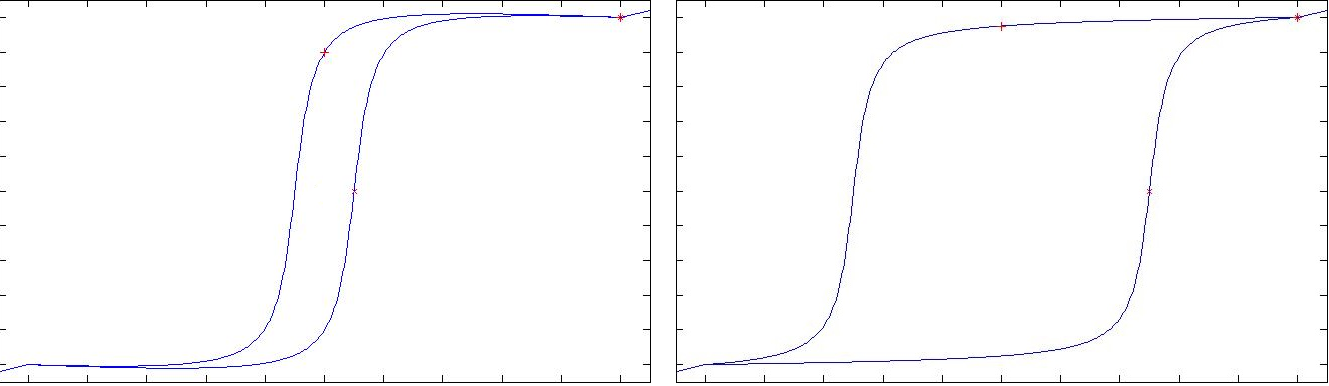
\includegraphics[scale=0.5]{images/histerese.png}
\end{center}
\legend{Curva de magnetização para material com pouca e muita histerese, respectivamente.}
\end{figure}
% ---
% Capitulo com exemplos de comandos inseridos de arquivo externo 
% ---
\chapter{Osciladores LC}
\label{osciladores-lc}
\chapterprecis{Em aplicações RF é mais comum empregar redes de realimentações utilizando somente tanques LC, devido ao alto fator de qualidade, podendo, também, assumir potências extremamentes altas (ao contrário, por exemplo, de redes com amplificadores operacionais). Alguns desses osciladores são: oscilador LC MOS, royer e mazzilli.}\index{sinopse de capítulo}
\section{Oscilador LC MOS cruzado acoplado}
Neste tipo de oscilador, os transistores estão em classe A, fornecendo energia ao tanque LC, consumida devido às perdas dos componentes. Neste caso, a energia que o transistor injeta no tanque, deve ser maior ou igual que a resistência de perda total do circuito. O fator de qualidade deste circuito é:
\begin{equation}
Q = \frac{2\pi f L}{R_p}
\end{equation}
E o $g_m$ é:
\begin{equation}
g_m = \frac{i_D}{V_{GS} - V_t}
\end{equation}
Para que ocorra uma oscilação:
\begin{equation}
\frac{1}{g_m} \geq \frac{2\pi f L}{Q}
\end{equation}
É importante notar que, mesmo que o circuito seja instável e os transistores entrem em corte e saturação, a tensão na saída continuará próxima de uma senoide para fatores de qualidade do tanque elevados.
Uma das grandes desvantagens desse circuito deve-se ao fato de que são poucos os MOSFETs que sustentam uma tensão de gate maior que 20V, limitando assim a potência do circuito.


\section{Oscilador Royer}
Em 1954, George Royer patenteou o oscilador Royer, um circuito auto ressonante, simples e com pouco uso de componentes. Como a maioria dos osciladores, ele utiliza um tanque LC para a oscilação. A grande vantagem deste circuito consiste no uso de um terceiro enrolamento conectado à base dos transistores, isto garante que um transistor estará cortado enquanto o outro estiver conduzindo, diminuindo drasticamente o consumo de energia do circuito.


\section{Oscilador Mazzilli}
O oscilador Mazzilli\cite{paolucci2009novel}\cite{mcclusky2010high} é uma derivação do oscilador Royer com o LC MOS. A grande diferença consiste no circuito presente no gate, para assegurar o baixo consumo energético e o chaveamento em ZVS\footnote{\emph{Zero-Voltage Switching} ocorre que o MOSFET só irá alternar de um estado para o outro quando a tensão do dreno for zero, reduzindo a perda, que normalmente é transformado em calor, do circuito} sem o uso de um terceiro enrolamento no indutor. O oscilador Mazzilli retira energia de Vin (como no Royer) e, no entanto, liga os gates, por meio de diodos, ao dreno oposto. Com isso, suprimos o problema de tensão que existia no LC MOS e continuamos a utilizar MOSFET ao invés de BJT, podendo assim, garantir alta frequência de oscilação.

\subsection{Modos de Operação}
%Esse conversor possui quatro modos de operação. O primeiro modo o dreno das duas chaves estão aterrados. Como a ligação é cruzada, garantimos que a chave 1 está cortada e a 2 ativa. Durante esta operação o capacitor é completamente descarregado. Depois disso a chave 1 é cortada e é a vez da chave 2 está ativa. Assim há a geração de uma corrente que irá percorrer o tanque LC e irá descarregar na chave ativa. Quando a voltagem no dreno 1 retorna para zero, ocorre o chaveamento das duas chaves. Assim como no modo de operação 1 o capacitor está completamente descarregado, e o indutor carrega totalmente a corrente em posição oposta. E finalmente, o modo 4 que ocorre exatamente o mesmo evento que o modo 2, no entanto, na chave 1.

Assumindo a chave 1 ativa e a chave 2 cortada temos o primeiro modo de operação. O dreno da chave 1 provê um aterramento para a corrente DC do circuito. Ambos os drenos estão com tensão zero, curto circuitando o capacitor. Toda energia do tanque está neste momento armazenada na corrente de pico do indutor. Como o circuito opera com ZVS, nenhuma corrente AC do tanque passa pelas chaves. Com a chave 2 cortada, o segundo modo de operação pode ser visto como a elevação e a queda da tensão do capacitor. A corrente no indutor carrega o capacior até a tensão máxima de dreno até a metade de tempo do segundo modo de operação do circuito. Com o pico da tensão de dreno em 2, toda a energia do ressonador é armazenado no capacitor. Após isto, o capacitor começa a se descarregar, transferindo a energia de volta para os indutores. O modo 3 mostrado na [], ocorre quando a tensão do nó 2 atinge zero. O MOSFET em push-pull é então chaveado, fornecendo um caminho para a corrente DC até o terra pela chave 2. Por fim, o último modo de operação ocorre de forma similar que o modo 2, no entando com a chave 2, como pode ser visto na [].

\subsection{Limitações do circuito}

\subsubsection{Dependência da carga}
Durante a transferência de potência a carga é refletida para o primário, e aparece em paralelo com o tanque LC, e com isso a frequência de oscilação é dependente da carga em uso, gerando uma perda maior.
\subsubsection{Resposta do Gate}
Quando a frequência de oscilação é baixa, este fator não é crucial. No entanto, com o aumento de frequência, o tempo de resposta do transistor pode interferir no funcionamento do circuito.

\subsubsection{Alta voltagem no Gate}
Outro problema é a alta voltagem presente no gate. Este problema é facilmente mitigado adicionando um zener com uma tensão ligeiramente abaixo da tensão de breakdown do gate, embora cause uma perda maior na resistência do gate.

\subsection{Resistência do transistor}
Quando o transistor está descarregando o capacitor, toda a corrente gerada no circuito passa através dele. Por isso, há a necessidade de optar por um MOSFET que possua a menor resistência possível quando ele estiver conduzindo, afim de manter a menor perda possível no transistor de forma a mitigar a dissipação de calor.
% ---

% ---
% Capitulo de revisão de literatura
% ---
\chapter{Experimento}
A primeira abordagem para realizar a montagem experimental foi construir uma placa de circuito impresso com o circuito do Mazzilli. Porém, o circuito planejado drenaria uma corente de 30A e oscilaria numa frequência em torno de 400kHz. Utilizando \cite{pcbtrace} para calcular qual deveria ser a espessura da trilha, chegamos a valores que não seriam práticos ($42$mm de espessura). Portanto a ideia era fazer a montagem em outro material e fazer as ligações por cabos que se usam em instalação elétrica, garantindo assim o funcionamento adequado. Para isto, foi feita a montagem experimental em cima de uma placa de madeira, que é um péssimo condutor, funcionando como um ótimo isolante. 
\section{Transistores}
Para podermos atender os requisitos citados no \autoref{osciladores-lc} foi necessário a escolha do IRFP250N, onde podemos conferir suas especificações na \autoref{tabela-car-irfp}.


\begin{table}[htb]
\IBGEtab{%
  \caption{Características do IRFP250N}%
  \label{tabela-car-irfp}
}{%
  \begin{tabular}{cccc}
  \toprule
   & Parâmetro & Valor & Unidade \\
  \midrule
  $I_{DMáx}$ & Corrente contínua de Dreno & $30$ & A \\
  $P_{DMáx}$ & Dissipação de potência & $214$ & W \\
  $V_{GS}$ & Tensão de gate para source & $\pm 20$ & V \\
  \bottomrule
\end{tabular}%
}{%
  \fonte{International Rectifier}%
  \nota{Os valores máximos são para uma temperatura de $25^oC$.}%
  \nota[Anotações]{* Existem os capacitores eletrolíticos bipolares porém não possuem capacitâncias tão altas.}%
  }
\end{table}


\section{Capacitores}
Outro problema prático é que o capacitor deve ser apolar, pois o sinal excursionado nele ora é positivo, ora é negativo. Além disto, a corrente AC que passa está na ordem de dezenas de amperes, havendo a necessidade de realizar associações em paralelo para dividir a corrente entre os componentes até um valor aceitável. A \autoref{tabela-cap-comp} mostra os materiais que são comumente fabricados o capacitor. Podemos observar que o melhor material para agir em conjunto com um circuito que irá oscilar em alta frequência, com uma alta tensão e maior fator de qualidade possível, é o polipropileno. No projeto, foi utilizado 3 capacitores, modelo B32653, de  $.22\mu F$ cada.


\begin{table}[htb]
\IBGEtab{%
  \caption{Comparativo entre os tipos de capacitores.}%
  \label{tabela-cap-comp}
}{%
  \begin{tabular}{cccccc}
  \toprule
  Tipo & Polaridade & Potência & Escala & ESR & Frequência de Operação \\
  \midrule
  Cerâmica & Não & Baixa & $\mu F$ & Baixo & Alta \\
  Poliestireno & Não & Alta & $pF$ & Baixo & Muito Alta \\
  Poliester & Não	& Alta & $\mu F$ & Baixo & Muito Alta \\
  Polipropilêno & Não & Alta & $\mu F$ & Muito baixo & Muito Alta \\
  Eletrolítico & Não* & Alta & $F$ & Alta & Baixa \\
  \bottomrule
\end{tabular}%
}{%
  \fonte{Wikipédia}%
  \nota{\hyphenation{Equivalent Series Resistence }: uma medida de não idealidade do componente que mede o valor da resistência em série com o mesmo para uma determinada frequência.}%
  \nota[Anotações]{* Existem os capacitores eletrolíticos bipolares porém não possuem capacitâncias tão altas.}%
  }
\end{table}



\section{Bobina de Trabalho}

\section{Choke}
Utilizando a fórmula aproximada de Wheeler \cite{wheeler1928simple}, adaptado em \cite{de2003calculo}, para ficar em metros e Henrys, temos que a fórmula explicita para o cálculo da indutância é:
\begin{equation}
L = \mu_0 \frac{\pi r^2 n^2}{h + 0.9r}
\end{equation}
Onde $ L$ é a indutância desejada, $\mu_0$ é a permeabilidade no ar, $r$ o raio da seção de reta do indutor, $n$ o número de espiras e $h$ a altura da bobina. Variando os parâmetros $r$, $h$ e $L$, considerando $h = 1.5r$, temos a Figura \ref{fig_comp-indutor}.

\begin{figure}[htb]
\caption{\label{fig_comp-indutor}Número de espiras variando os parâmetros para um indutor de núcleo de ar}
\begin{center}
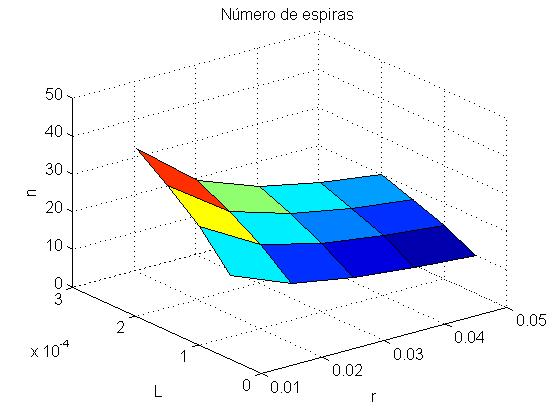
\includegraphics[scale=0.5]{images/comp-indutor.jpg}
\end{center}
\legend{O raio está variando de 1 a 5cm, enquanto a indutância varia de 50 a 200 $\mu H$ }
\end{figure}

Podemos observar que para uma bobina pequena temos que aumentar exponencialmente o número de espiras, além de tomar todo o cuidado para termos um espaçamento e seção de reta uniforme em cada espira. Para sanar o problema, recorremos ao uso de choques com núcleo de ferrite, comumente encontrado em fontes chaveadas. O ferrite possuí como característica alta permeabilidade magnética, baixa condutividade elétrica (prevenindo correntes parasitas) e baixa perda em alta frequência, garantido assim um menor $n$ e consequentemente um menor tamanho de choque. Encontramos a bobina em uma fonte ATX, muito utilizada em computadores (ver \autoref{fig_fonte-atx}).

\begin{figure}[htb]
\caption{\label{fig_fonte-atx}Demonstração do choke na fonte ATX}
\begin{center}
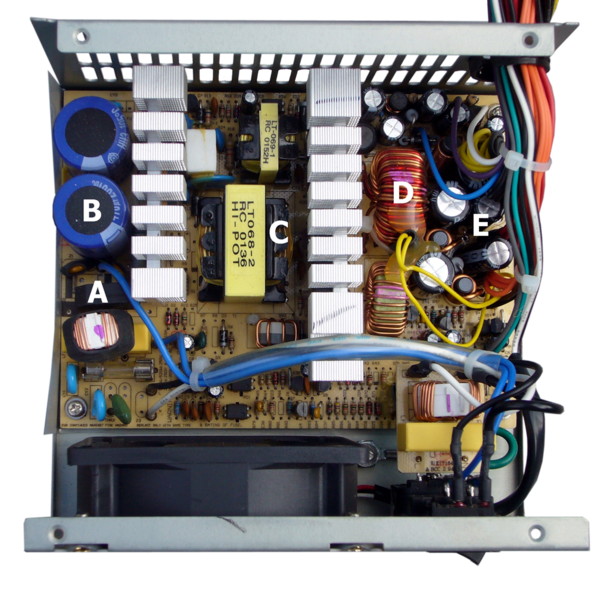
\includegraphics[scale=0.5]{images/fonte-atx.png}
\end{center}
\legend{Observe o choke, marcado com a letra 'D', de uma fonte ATX com núcleo de ferrite enrolado com várias espiras. Fonte: Wikipedia.}
\end{figure}


\section{Diodo de recuperação rápida}
O diodo que realiza o chaveamento do transistor no momento certo, ajudando a descarregar a base, deve poder responder na mesma velocidade de chaveamento necessária no circuito, com isso utilizamos o diodo BYV26A, que tem como principais aplicações, inversores em alta frequência e fontes chaveadas.
\section{Fonte}
Um dos fatores cruciais do projeto é a fonte de alimentação. Ela deve ser capaz de fornecer uma energia de 200W, uma corrente de 20A e ideal seria uma tensão regulada. No entanto, como o projeto em si é uma prova de conceito, não foi possível conseguir uma fonte de tensão regulável. Por fim, utilizamos uma bateria de chumbo, modelo FP12180, de 18Ah, mostrada na \autoref{fig_bateria}.

\begin{figure}[h]
\caption{\label{fig_bateria}Montagem experimental}
\begin{center}
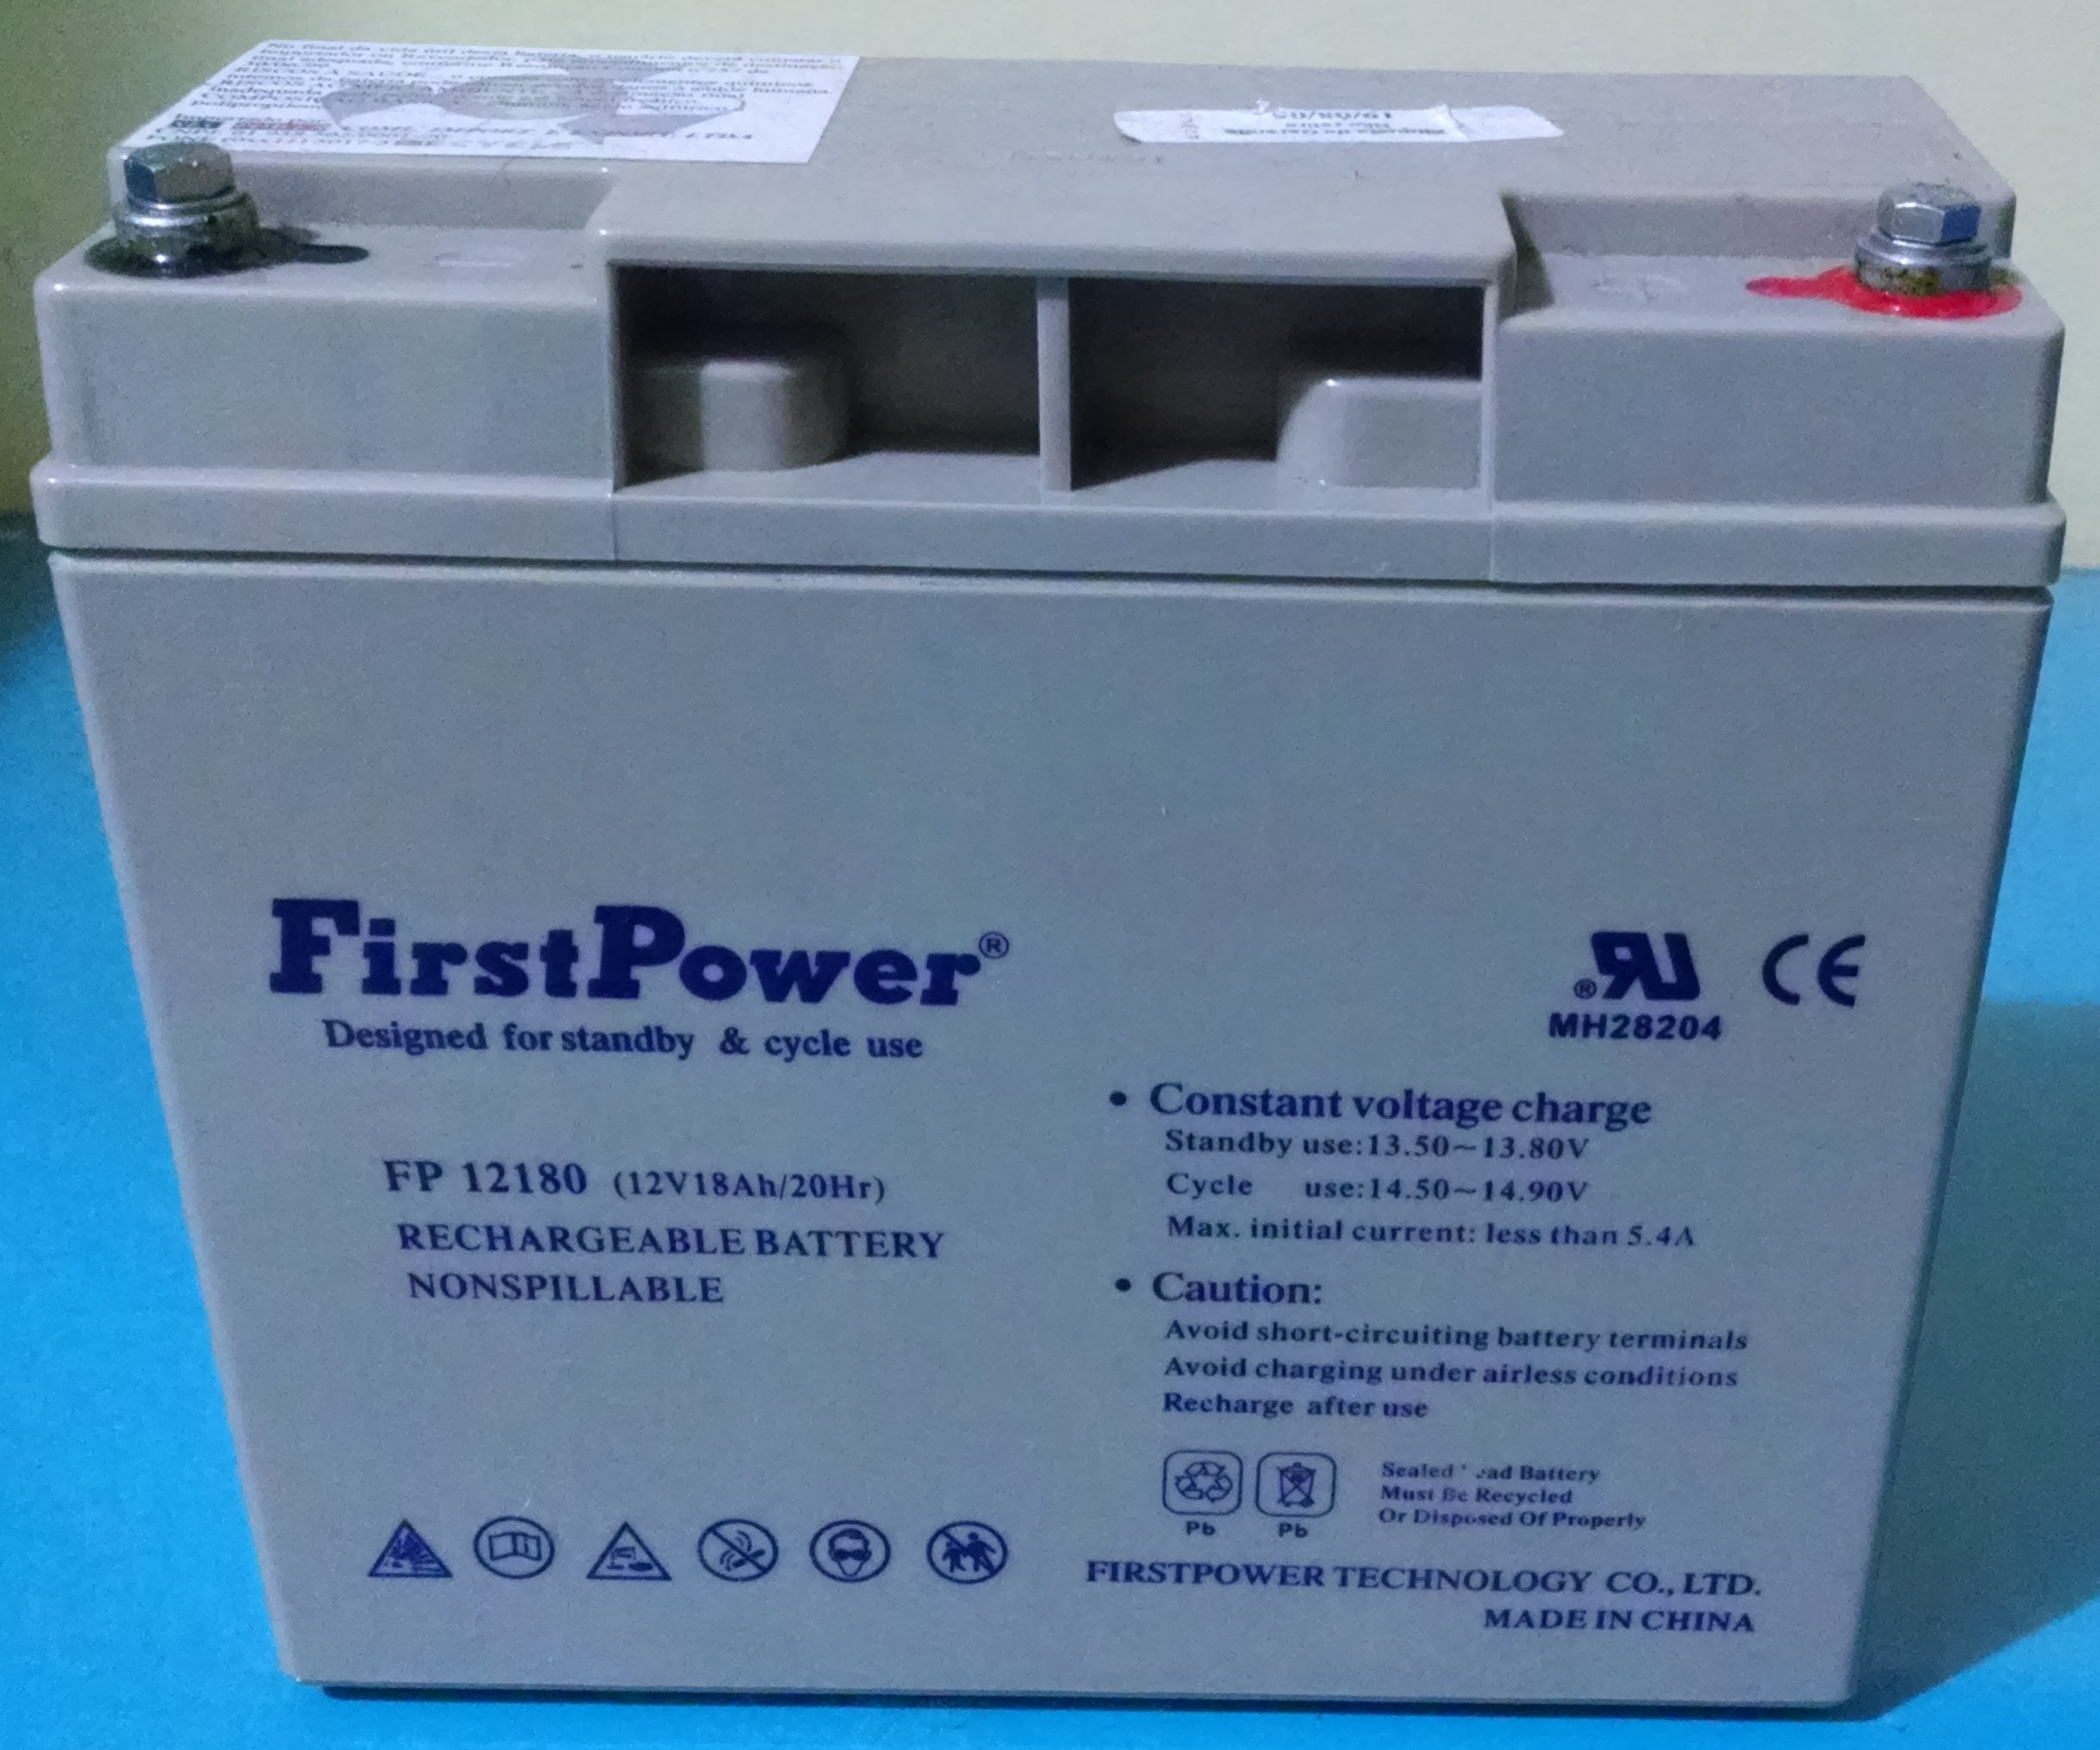
\includegraphics[scale=0.1]{images/bateria.jpg}
\end{center}
\legend{Montagem experimental do circuito na base de madeira.}
\end{figure}

\section{Montagem}
Utilizamos solda de estanho e fios de $1\mbox{mm}^2$ e $1.5\mbox{mm}^2$ para a parte de baixa e alta tensão, respectivamente. A montagem final pode ser conferida na \autoref{fig_montagem}.

\begin{figure}
\caption{\label{fig_montagem}Montagem experimental}
\begin{center}
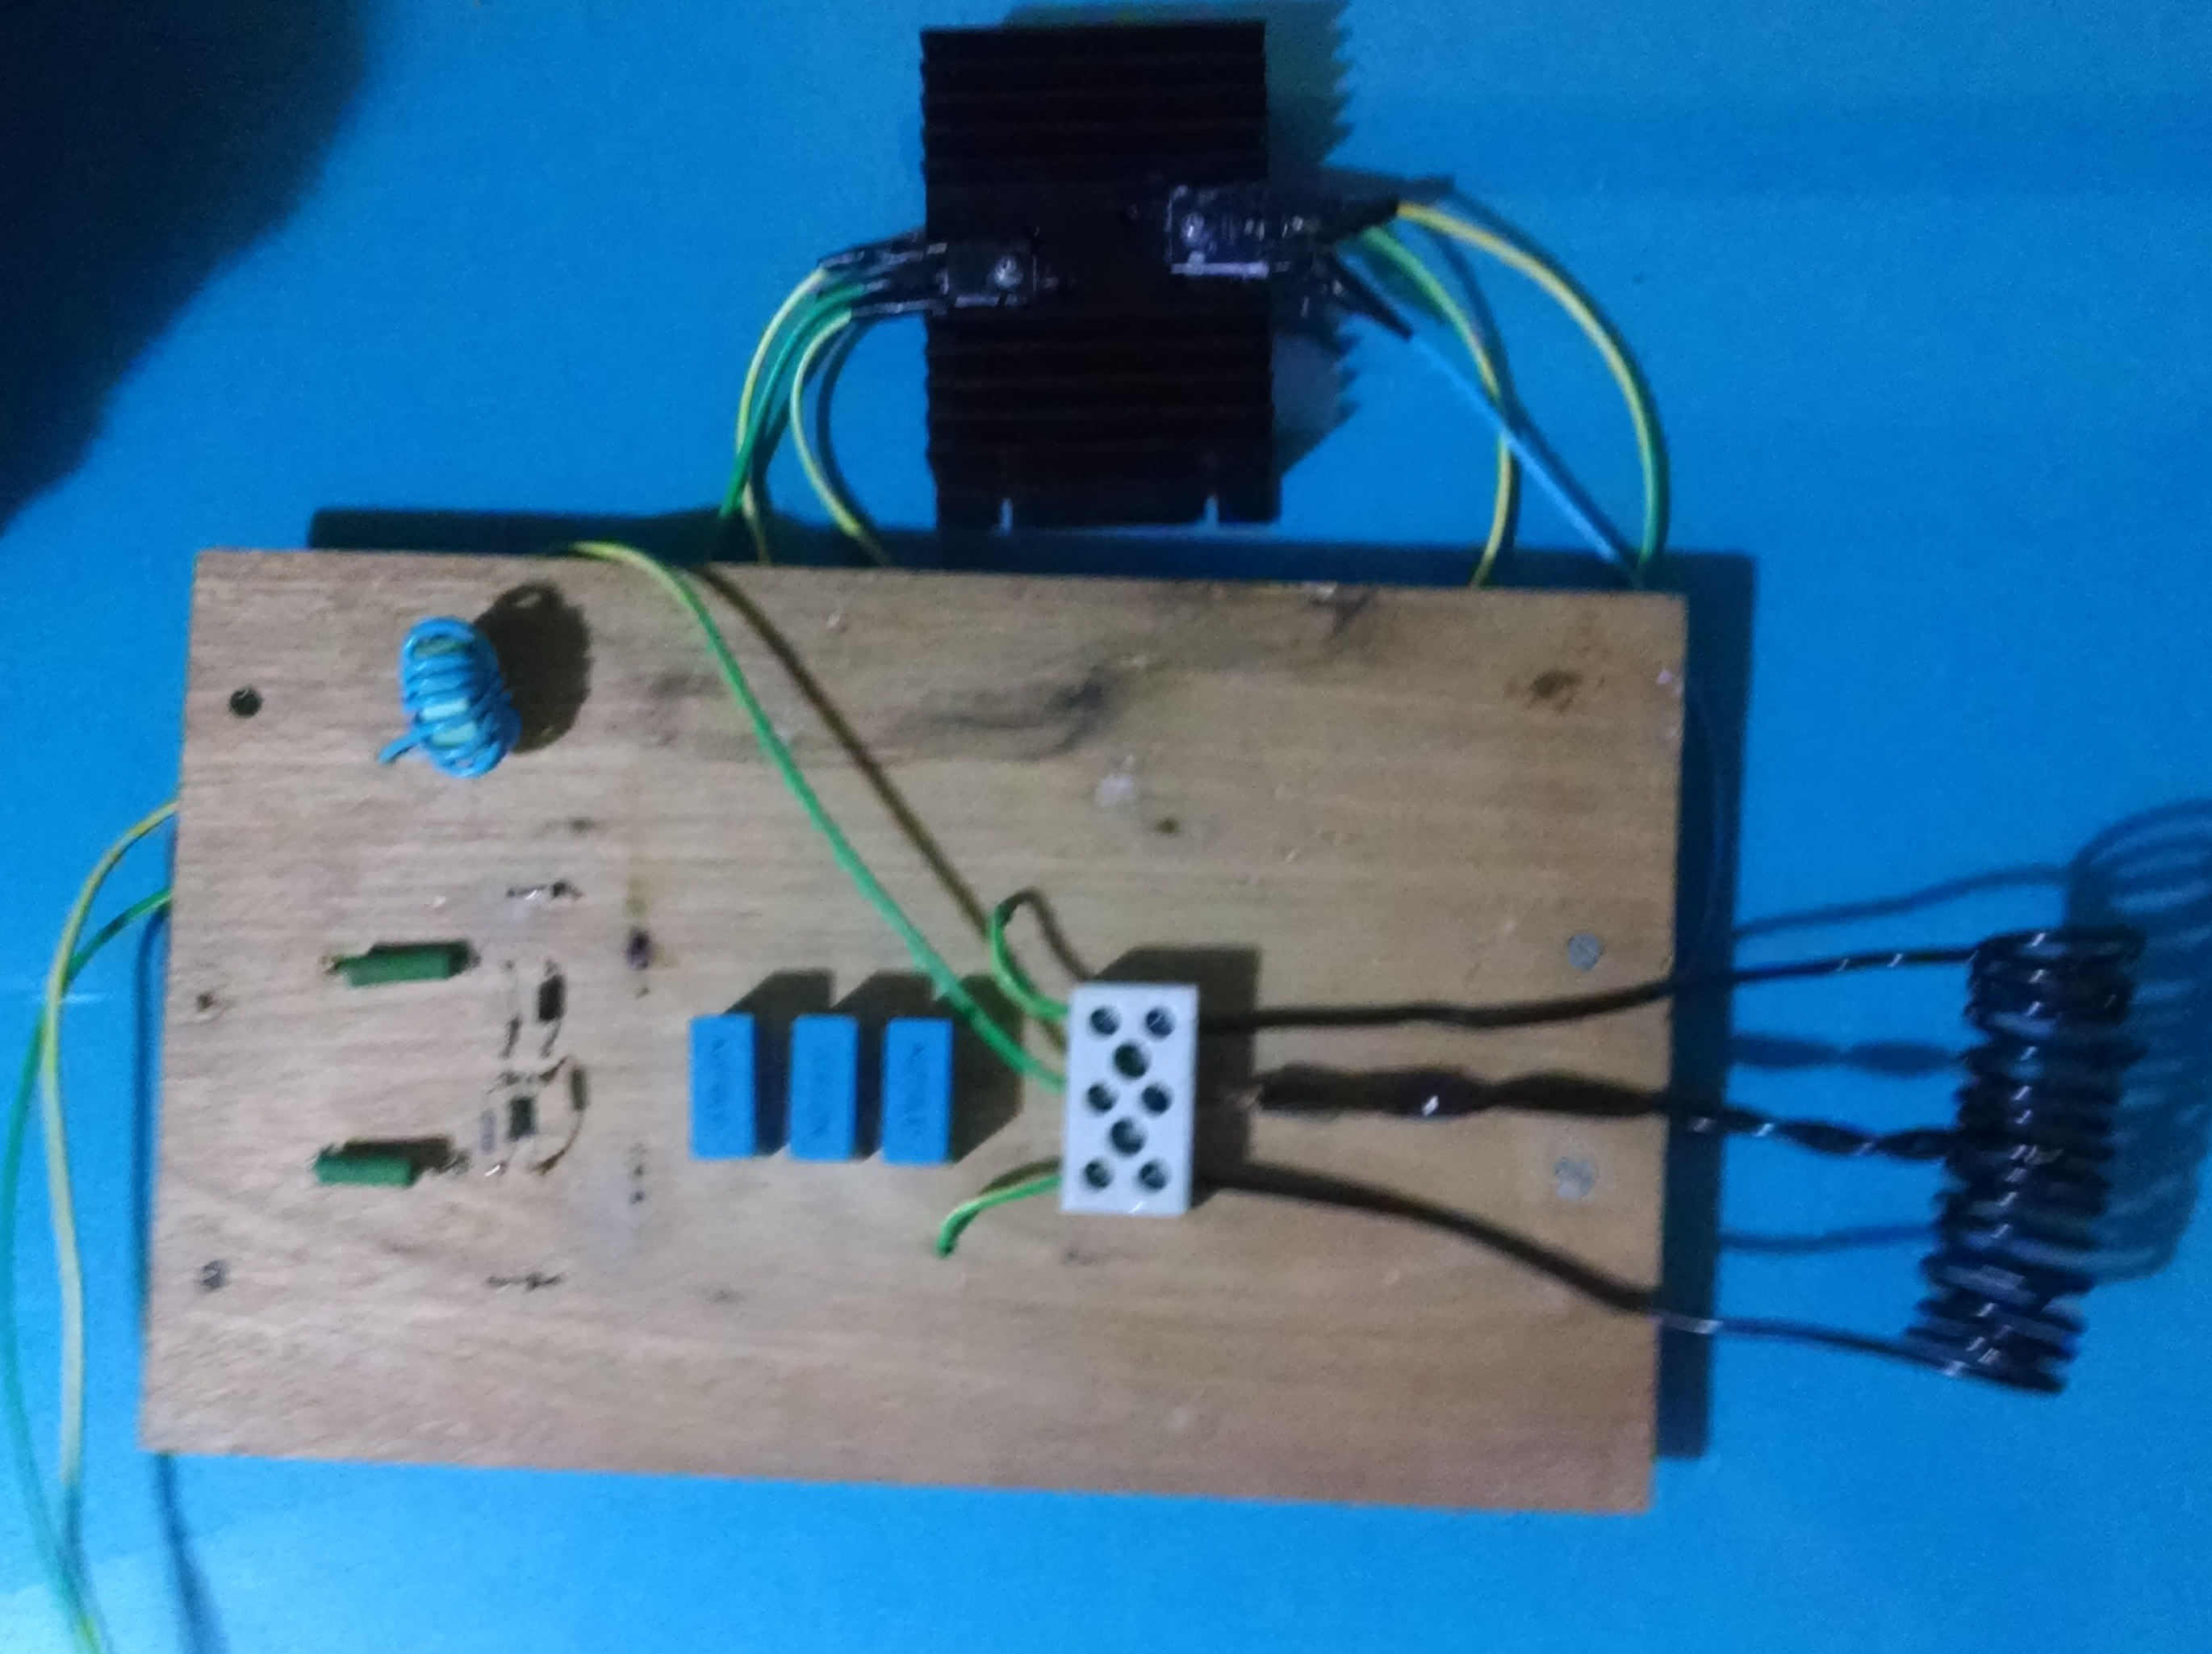
\includegraphics[scale=0.1]{images/montagem.jpg}
\end{center}
\legend{Montagem experimental do circuito na base de madeira. Fios de cor amarela são de $1\mbox{mm}^2$ enquanto os verdes são de $1.5\mbox{mm}^2$}
\end{figure}
% ---



% ----------------------------------------------------------
% Finaliza a parte no bookmark do PDF
% para que se inicie o bookmark na raiz
% e adiciona espaço de parte no Sumário
% ----------------------------------------------------------
\phantompart

% ---
% Conclusão (outro exemplo de capítulo sem numeração e presente no sumário)
% ---
\chapter{Resultados}
Após realizarmos testes no circuito montado, verificamos que o circuito de fato aquecia objetos metálicos. No entanto, devido à operação em potência relativamente baixa, apenas materiais ferromagnéticos tiveram aquecimento expressivo, o que nos leva a concluir que o efeito de histerese é o principal fator para o aquecimento. As correntes de Foucault não dissipam calor significativo mesmo após exposição prolongada ao campo eletromagnético. Foram feitos testes com ferro, alumínio e cobre e apenas materiais de ferro foram aquecidos.

Devido a limitações de tensão da fonte, não foi possível a operação em potências maiores que $216$W, já que com tensão de apenas $12$V, a corrente ficaria demasiadamente elevada. Testes com correntes mais altas levaram a danos nos transistores, que tiveram que ser substituídos.

Apesar do limite de potência, pudemos validar o experimento como prova de conceito, e imaginamos que com potências da ordem de grandeza de um chuveiro elétrico convencional, um chuveiro por aquecimento indutivo seja realizável.
% ---


% ----------------------------------------------------------
% ELEMENTOS PÓS-TEXTUAIS
% ----------------------------------------------------------

% ----------------------------------------------------------

% ----------------------------------------------------------
% Referências bibliográficas
% ----------------------------------------------------------
\bibliography{referencias}

% ----------------------------------------------------------
% Glossário
% ----------------------------------------------------------
%
% Consulte o manual da classe abntex2 para orientações sobre o glossário.
%
%\glossary

% ----------------------------------------------------------
% Apêndices
% ----------------------------------------------------------

% ---
% Inicia os apêndices
% ---
%\begin{apendicesenv}
%
%% Imprime uma página indicando o início dos apêndices
%\partapendices
%
%% ----------------------------------------------------------
%\chapter{Quisque libero justo}
%% ----------------------------------------------------------
%
%
%% ----------------------------------------------------------
%\chapter{Nullam elementum urna vel imperdiet sodales elit ipsum pharetra ligula
%ac pretium ante justo a nulla curabitur tristique arcu eu metus}
%% ----------------------------------------------------------
%
%\end{apendicesenv}
% ---


% ----------------------------------------------------------
% Anexos
% ----------------------------------------------------------

% ---
% Inicia os anexos
% ---
%\begin{anexosenv}
%
%% Imprime uma página indicando o início dos anexos
%\partanexos
%
%% ---
%\chapter{Morbi ultrices rutrum lorem.}
%% ---
%
%% ---
%\chapter{Cras non urna sed feugiat cum sociis natoque penatibus et magnis dis
%parturient montes nascetur ridiculus mus}
%% ---
%
%
%% ---
%\chapter{Fusce facilisis lacinia dui}
%% ---
%
%
%\end{anexosenv}

%---------------------------------------------------------------------
% INDICE REMISSIVO
%---------------------------------------------------------------------
\phantompart
\printindex
%---------------------------------------------------------------------

\end{document}
